\begin{frame}[fragile]{man chmod}
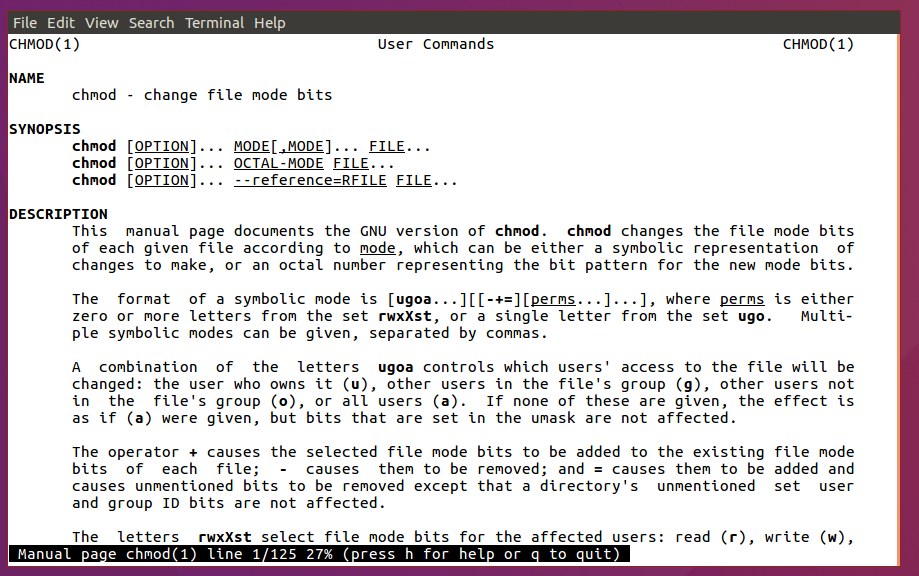
\includegraphics[width=.95\textwidth]{../commandLineTips/manchmod}
\end{frame}

\begin{frame}[fragile]{chmod}
\begin{tikzpicture}
\node (exampleCmd) {
    \strut\verb|chmod| 
}; 
\node[right=2mm of exampleCmd,baseline=exampleCmd.base] (optR) {
    \strut\verb|--recursive|
};
\node[right=2mm of optR,baseline=exampleCmd.base] (opt) {
    \strut\verb|og-r|
};
\node[right=2mm of opt,baseline=exampleCmd.base] (files) {
    \strut\verb|/home/USER|
};

\onslide<2|handout:0>{
    \node[below=1cm of opt, align=center] (optExplain) {
        \myemph{o}thers and \myemph{g}roup (student) \\ 
        {\color{red}\texttt{-}} remove \\
        \myemph{r}ead
    };
}
\onslide<2-3>{
    \begin{pgfonlayer}{bg}
    \node[fit=(opt),rounded corners=3pt,fill=blue!20!white,inner sep=0mm] {};
    \end{pgfonlayer}
}

\onslide<3>{
    \node[below=1cm of opt, align=center] {
        \myemph{u}ser (yourself) / \myemph{g}roup / \myemph{o}thers \\
        {\color{red}\texttt{-}} remove / {\color{red}\texttt{+}} add \\
        \myemph{r}ead / \myemph{w}rite / e\myemph{x}ecute or search
    };
}

\end{tikzpicture}
\end{frame}
